\begin{figure}[htbp]
\centering
\begin{minipage}[c]{.46\textwidth}
\centering
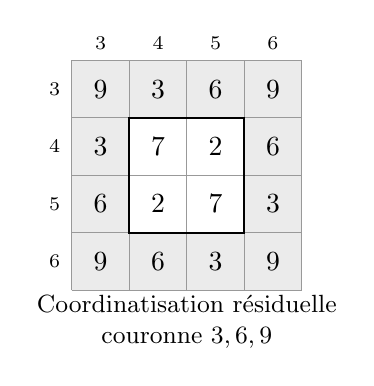
\begin{tikzpicture}[x=.73cm,y=.73cm]
\fill[black!8] (0,0) rectangle (4,4);
\fill[white] (1,1) rectangle (3,3);
\draw[step=1,black!40] (0,0) grid (4,4);
\draw[thick] (1,1) rectangle (3,3);
\foreach \row/\vals in {0/{9,3,6,9},1/{3,7,2,6},2/{6,2,7,3},3/{9,6,3,9}}{
  \foreach \val [count=\col from 0] in \vals{
    \node at (\col+.5,3.5-\row) {\(\val\)};
  }
}
\foreach \v [count=\n from 0] in {3,4,5,6}{
  \node[font=\scriptsize] at (\n+.5,4.3) {\(\v\)};
  \node[font=\scriptsize] at (-.3,3.5-\n) {\(\v\)};
}
\node[font=\small,align=center] at (2,-.55) {Coordinatisation résiduelle\\couronne \(3,6,9\)};
\end{tikzpicture}
\end{minipage}\hfill
\begin{minipage}[c]{.50\textwidth}
\centering
\begin{tikzpicture}[x=.73cm,y=.73cm]
\fill[black!3] (0,0) rectangle (4,4);
\draw[black!40] (0,0) rectangle (4,4);
\draw[thick] (1,1) rectangle (3,3);
\foreach \x/\y/\v in {.5/3.5/9,3.5/3.5/18,.5/.5/18,3.5/.5/36,
  1.5/2.5/16,2.5/2.5/20,1.5/1.5/20,2.5/1.5/25}{
  \node at (\x,\y) {\(\v\)};
}
\draw[-{Stealth},black!60] (.85,3.15) -- (1.22,2.78);
\draw[-{Stealth},black!60] (3.15,3.15) -- (2.78,2.78);
\draw[-{Stealth},black!60] (.85,.85) -- (1.22,1.22);
\draw[-{Stealth},black!60] (3.15,.85) -- (2.78,1.22);
\node[font=\small,align=center] at (2,-.55) {Frontière relevée\\et interpolation multiaffine};
\end{tikzpicture}
\end{minipage}
\caption{La même coordinatisation selon deux lectures. À gauche, la couronne radicale entoure le bloc \(B_c\). À droite, les quatre sommets entiers déterminent les valeurs intérieures sous la loi multiaffine. Leurs résidus aux sommets coïncident, mais les quotients \((0,1,1,3)\) distinguent le relèvement.}
\label{fig:centro-frontera}
\end{figure}
